\section{Analyse des Datensatzes}

In der Sektion~\ref{feature_extraction} wird der Datensatz verarbeitet und mit den in Tabelle~\ref{tab:features} erweitert.
In diesem Abschnitt wird das Resultat der Sektion~\ref{feature_extraction} analysiert.
Für den weiteren Verlauf der hier vorgestellten Methode wird die Skriptsprache Python in Kombination mit Jupyter-Notebooks benutzt. Für die Analyse der Daten wird Python-Bibliothek pandas verwendet. Für die Visualisierung durch verschiedene Arten von Diagrammen wird die Python-Bibliothek plotly eingesetzt.


\begin{table}[h]
    \begin{tabular}{|c|c|}
        \hline
        Entwurfsmuster & Anzahl\\
        \hline
        Singleton&15\\Adapter&9\\Command&8\\Observer&6\\Strategy&6\\Iterator&6\\Factory Method&5\\Template Method&5\\Composite&5\\Proxy&4\\Memento&4\\Builder&4\\Visitor&4\\State&3\\Abstract Factory&3\\Decorator&2\\Facade&1\\Bridge&1\\Null Object&1\\Prototype&1\\FactoryMethod&1\\Mediator&1\\
        \hline
    \end{tabular}
    \caption{Verteilung der Entwurfsmuster in P-MArt}
    \label{tab:dp_dist}
\end{table}



Die Tabelle~\ref{tab:dp_dist} zeigt die Verteilung der Instanzen der Design Pattern an. 
Dabei ist abzulesen, dass die Singelton-, Adapter-, Command- und Observer-Entwurfsmuster die am häufigsten vertretenen Entwurfsmuster sind, während Instanzen der Design Patterns wie Decorator oder Bridge nur einmal vorkommen.

\pagebreak

\begin{figure}[h]
    \centering
    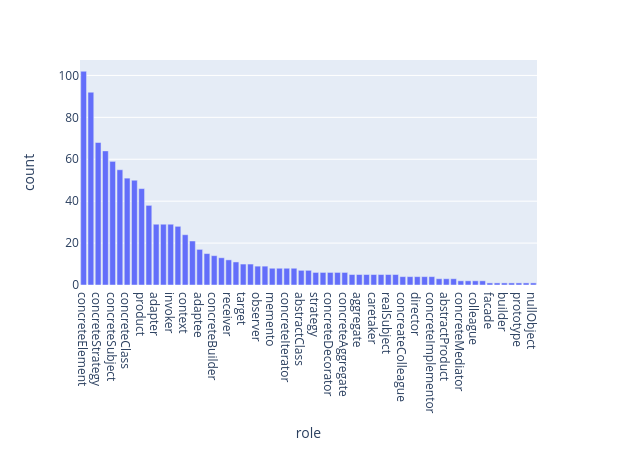
\includegraphics[scale=0.6]{figures/role_dist.png}
    \caption{Rollenverteilung in P-MArt}
    \label{fig:role_dist}
\end{figure}

Abbildung~\ref{fig:role_dist} ermöglicht einen Überblick über die Rollenverteilung.
Dabei ist zu vermerken, dass die Verteilung der Rollen und die Anzahl der Instanzen der zugehörigen Design Pattern unbalanciert ist. Beispielsweise ist die Rolle \textit{concreteelement} des Visitor-Entwurfsmusters am häufigsten vorzufinden, obwohl in P-MArt vier Instanzen vermerkt sind.
Um ein möglichst aussagekräftiges Ergebnis zu erhalten, muss die Menge der zu identifizierenden Entwurfsmuster eingeschränkt werden. Ansonsten ist bei zu vielen identifizierbaren Klassen mit wenigen Datenpunkten eine unzufriedenstellende Leistung der Klassifizierer zu erwarten.
Deshalb werden im weiteren Verlauf Instanzen der Entwurfsmuster Singelton, Observer, Command und Adapter weiter betrachtet.


\begin{table}[H]
    \begin{tabular}{|c|c|c|}
        \hline
        Entwurfsmuster & Rolle & Anzahl\\
        \hline
        Singelton & singelton & 15\\
        \hline
        \multirow{4}{*}{Adapter} & adaptee & 17\\ & adapter & 29\\ & client & 13\\ & target & 10\\
        \hline
        \multirow{5}{*}{Command} & client & 13\\ & command & 6\\ & concreteCommand & 50\\ & invoker & 29\\ & receiver & 12\\
        \hline
        \multirow{4}{*}{Observer} & concreteObserver & 28\\ & concreteSubject & 59\\ & observer & 9\\ & subject & 5\\
        \hhline{|=|=|=|}
        Insgesamt & & 295\\
        \hline
    \end{tabular}
    \caption{Aufteilung des Datensatzes für Training und Validierung}
    \label{tab:dataset_dist}
\end{table}

Tabelle~\ref{tab:dataset_dist} zeigt den Datensatz an, der im weiteren Verlauf verwendetet wird. Auf vier Design Pattern aufgeteilt,
beträgt der Umfang des Datensatzes 295 Datenpunkte auf vierzehn Rollen aufgeteilt.

\begin{figure}[h]
    \centering
    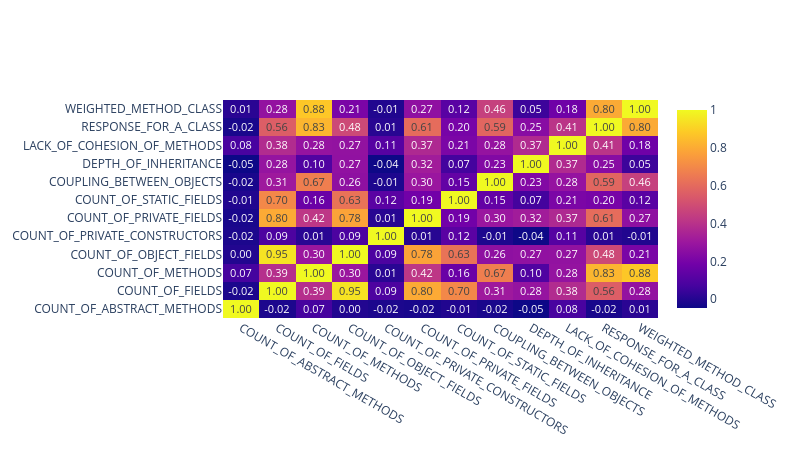
\includegraphics[scale=0.5]{figures/coff_heat_map.png}
    \caption{Koeffizienten-Heatmap der Features}
    \label{fig:coeff_heat_map}
\end{figure}

\pagebreak

Abbildung~\ref{fig:coeff_heat_map} beschreibt die Koeffizienten der Korrelation der einzelnen Features zueinander. Der Koeffizient der Korrelation wird paarweise für jede Metrik ermittelt.
Dabei kann der Koeffizient wie gefolgt interpretiert werden:

\begin{itemize}
    \item Zwischen -1.0 und 0: Dies wird als eine negative Korrelation bezeichnet. Je größer der eine Wert, desto kleiner wird der andere. Je kleiner der Koeffizient, desto größer der Einfluss.
    \item Gleich 0: Keine Korrelation ist vorzufinden.
    \item Zwischen 0 und 1.0: Ein Koeffizient in diesem Wertebereich wird als positive Korrelation benannt. Je größer der eine Wert, desto größer wird der andere. Je größer der Koeffizient, desto größer der Einfluss.
\end{itemize}

Bei der Datenanalyse von Features kann eine Koeffizienten-Heatmap dazu verwendet, um gegebenenfalls Features aus dem Featurevektor, um dessen Dimensionalität zu reduzieren. Die Dimensionalität beschreibt in diesem Kontext Anzahl der Komponenten im Featurevektor.
Je höher die Dimensionalität, desto mehr Möglichkeiten müssen berücksichtigt werden, um im Falle der Klassifikation eine möglichst passende Klasse zuzuordnen. Je kleiner die Dimensionalität, desto präziser kann klassifiziert werden.
Features mit einer besonders geringen oder hohen Koeffizient der Korrelation zu einer anderen encodieren ähnliche oder gleiche Informationen über die Entität, weshalb diese unter Umständen nicht mehr als Eingabe für Klassifizierer berücksichtigt werden.
Im Falle der Heatmap aus Abbildung~\ref{fig:coeff_heat_map} sind besonders hohe Koeffizienten der Korrelation vorzufinden. Jedoch werden unter Berücksichtigung des Domainwissens die alle Features für die Klassifikation verwendet
  



